\chapter{Introduction}
\label{chapter_introduction}
%% Start the actual chapter on a new page.
\newpage

\noindent

Once upon a time, there was the first living organism, the 
First Universal Common Ancestor (FUCA).
We do not know when it lived.

\begin{figure}[H]
  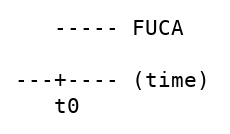
\includegraphics[width=0.2\textwidth]{t_0.png}
  % 
  %    ----- FUCA
  %
  % ---+---- (time)
  %    t0
  %
  \caption{
    Evolutionary history of the First Universal Common Ancestor (FUCA).
    Time goes from past (left) towards the present (right).
    \richel{TODO: Use proper phylogeny with proper timescale}
  }
  \label{fig:t_0}
\end{figure}

One unknown day, FUCA speciated, resulting in two species.
This event doubled the biodiversity on Earth.
The two species, which we will call species A and B
are sister species.
We do not know what caused the speciation.

\begin{figure}[H]
  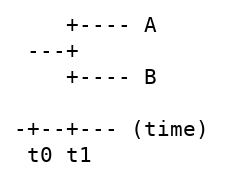
\includegraphics[width=0.2\textwidth]{t_1.png}
  %
  %     +---- A
  %  ---+
  %     +---- B
  %
  % -+--+--- (time)
  %  t0 t1
  %
  \caption{
    Evolutionary history of the First Universal Common Ancestor (FUCA).
    and its two decendants.
    Time goes from past (left) towards the present (right).
    \richel{TODO: Use proper phylogeny with proper timescale}
  }
  \label{fig:t_1}
\end{figure}

Both species A had their unknown histories: they speciated themselves,
and they and/or their descendants went extinct. 
Extinction is a common event. Let's assume A and/or its clade went
exctint and that species B created a sister species C. Species B
and C will give rise to all contemporary biodiversity. This ancestor of species B and C 
is called the Last Universal Common Ancestor and lived around [then].

\begin{figure}[H]
  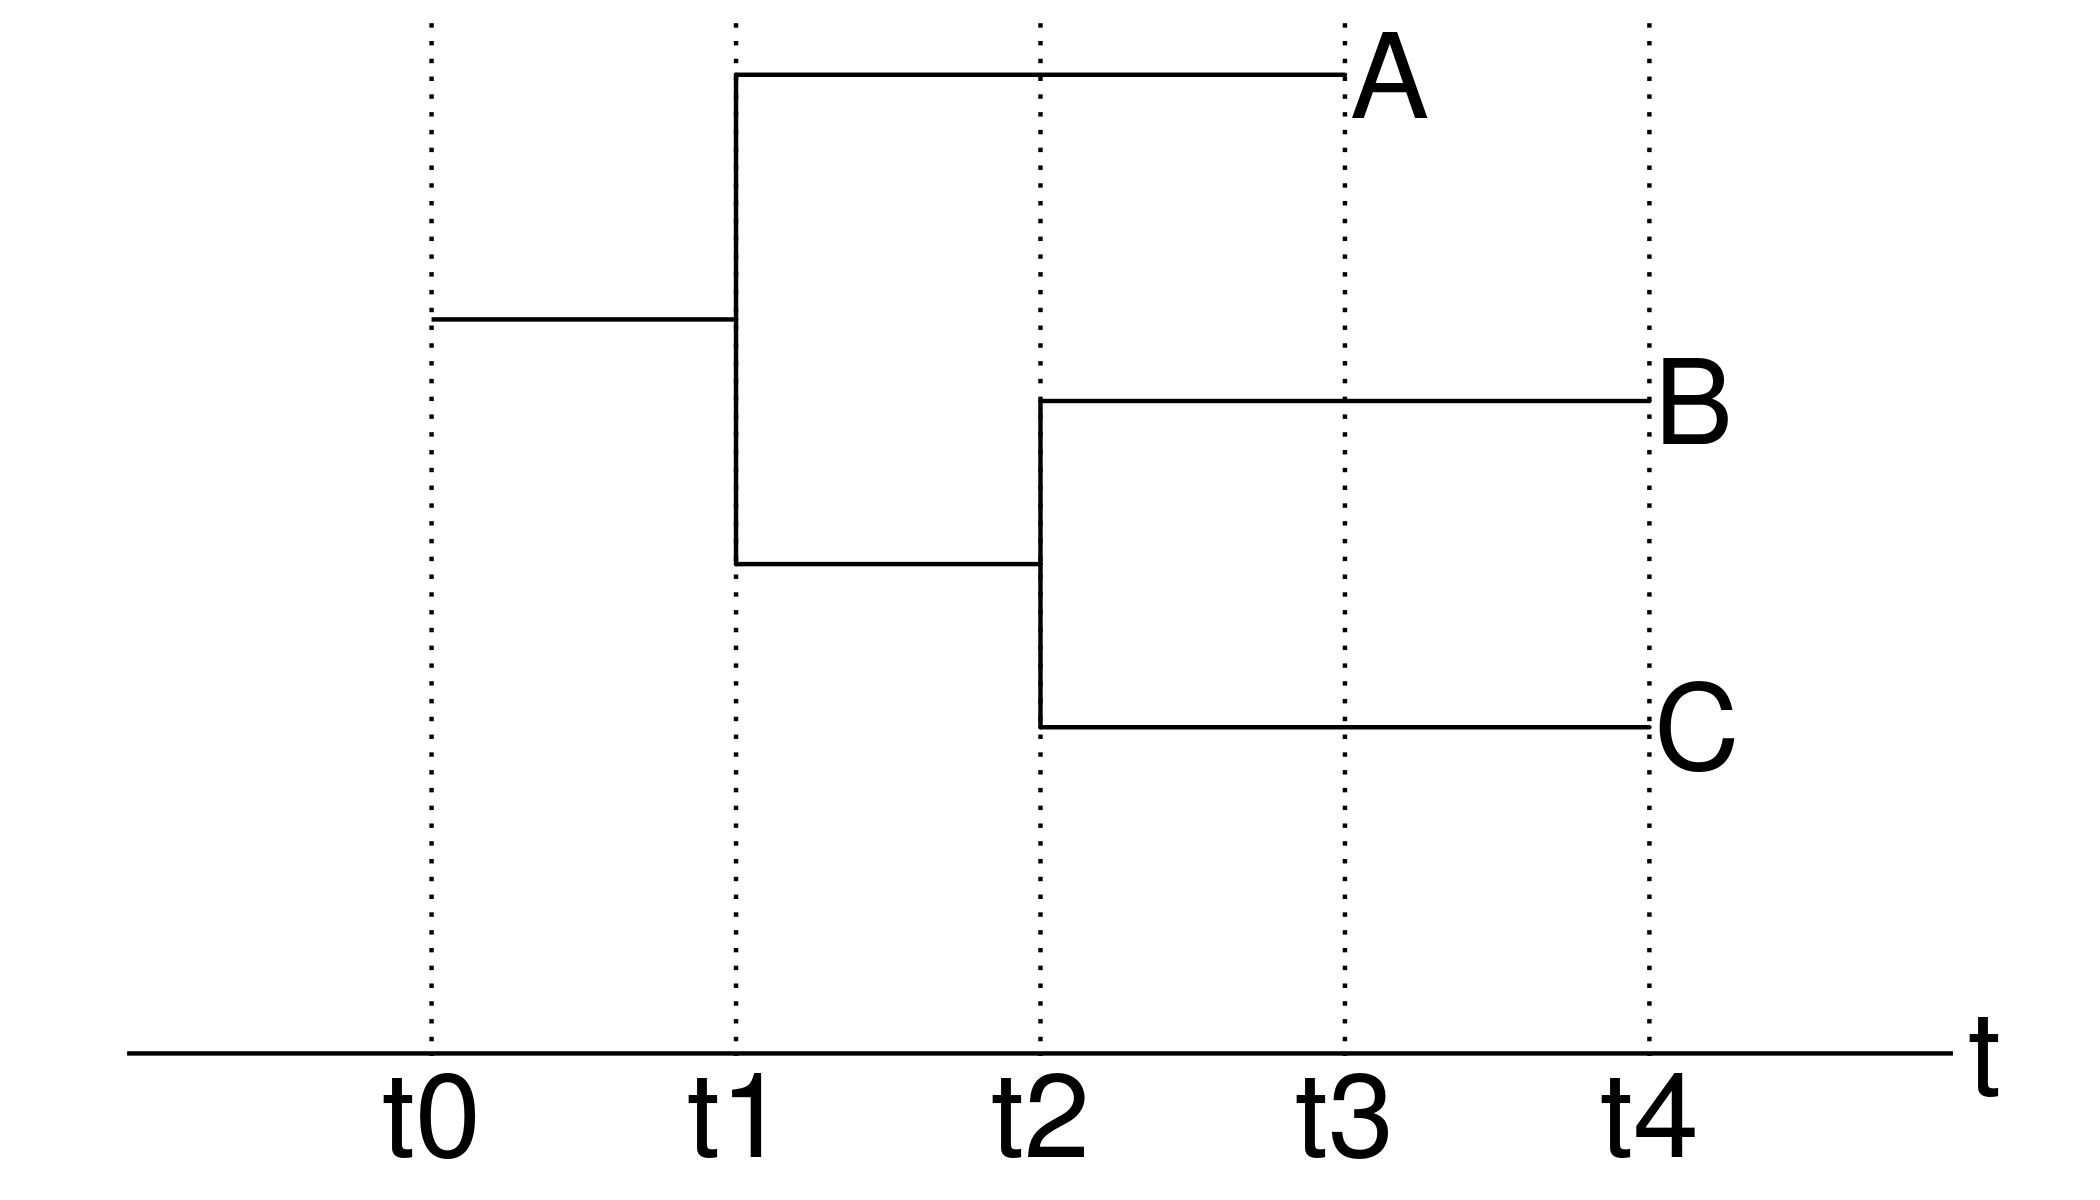
\includegraphics[width=0.4\textwidth]{t_3.png}
  %
  %     +--------x   A
  %  ---+     
  %     |     +------- B
  %     +-----+
  %           +------- C
  %
  % -+--+-----+--+---- (time)
  %  t0 t1    t2 t3
  %
  \caption{
    Evolutionary history of the First Universal Common Ancestor (FUCA).
    and its three decendants of which one went extinct.
    Time goes from past (left) towards the present (right).
    Assuming B and C will give rise to all contemporary biodiversity,
    the Last Universal Common Ancestor (LUCA) must have come into existence
    at timepoint t1.
    \richel{TODO: Use proper phylogeny with proper timescale}
  }
  \label{fig:t_3}
\end{figure}

The biodiversity derived from LUCA is important to us 
humans (apart from that is has created us) for many reasons.
Biodiversity is found so important, that, for example, 
the European Union has an explicit Biodiversity Strategy,
which aims to halt the loss of biodiversity and ecosystem 
services (\url{https://ec.europa.eu/environment/nature/biodiversity/strategy/index_en.htm}).
Ecosystem services are features of biological systems that are 
positive for human well-being, for example food,
carbon sequestration, waste decomposition and pest control.
A review paper \cite{cardinale2012biodiversity} shows that 
biodiversity unsually improves ecosystem services.

\begin{figure}[H]
  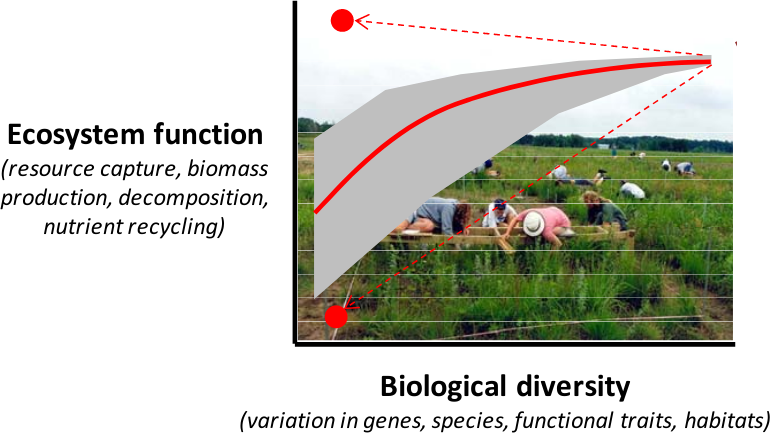
\includegraphics[width=0.5\textwidth]{cardinale_et_al_fig_1.png}
  %
  % Ecosystem function
  %
  %   |  _______
  %   | /
  %   |/
  %   +--------------
  %
  %     Biological diversity
  \caption{
    A diversity-function relationship found to be typical from hundreds
    of studies. The red line represents an average, where the grey polygon
    represents a 95\% confidence interval. The red dots show the lower
    and upper limit for monocultures. From \cite{cardinale2012biodiversity}
  }
  \label{fig:cardinale_et_al}
\end{figure}


Speciation is the process that increases biological diversity.
This process is studied from multiple angles, among others,
we can study the mechanism ('what
causes a speciation event?') or we can study the patterns of many
of such events ('is speciation rate constant through time?')

%
% [picture of speciation machanism] | [picture of a trait that increases speciation rate]
%                                   | 
% Speciation mechanism:             | Speciation events though time:                           
% what caused this speciation       | what are the patterns of
% event to occur?                   | speciation events?
% In this case, a geographics       | In this case, a trait that was a key innovation
% barrier caused the initial        | gave rise to a higher speciation rate
% species to diverge                | 
%

The mechanism of a speciation event has many facets.
For more than half a century ago, it was hypothesized
that speciation is caused by geographical isolation (e.g. Mayr, 1942)
or due to ecological factors (e.g. Lack, 1947).

% [picture of geographical isolation] | [picture of ecological factors]
% [from Mayr's paper]                 | [the Darwin finches of course!]
%                                     |
% Speciation can happen due to        | Speciation can happen due to
% a geographic barrier                | ecological factors
%

Instead of looking at the mechanism behind each speciation event,
we can also look at patterns of speciation events through evolutionary time,
asking question such as 'How often do speciation and extinction events take place?'
'Are speciation and extinctions rates constant or do they change?',
'What causes a change in speciation or extinction rate?' or
'Is there an upper limit on the number of species?'.

There are two methods to research speciation patterns back in evolutionary time:
the use of fossils or using molecular phylogenies.

\begin{figure}[H]
  %
  % [picture of El Graeco fossil] | [](800px-Hominini_lineage.svg.png), from https://en.wikipedia.org/wiki/File:Hominini_lineage.svg
  %                               | 
  %  El Greaco                    | HS     Pan
  %                               |  \    /
  %                               |   \  /
  %                               |    \/
  %                               |     \
  %
  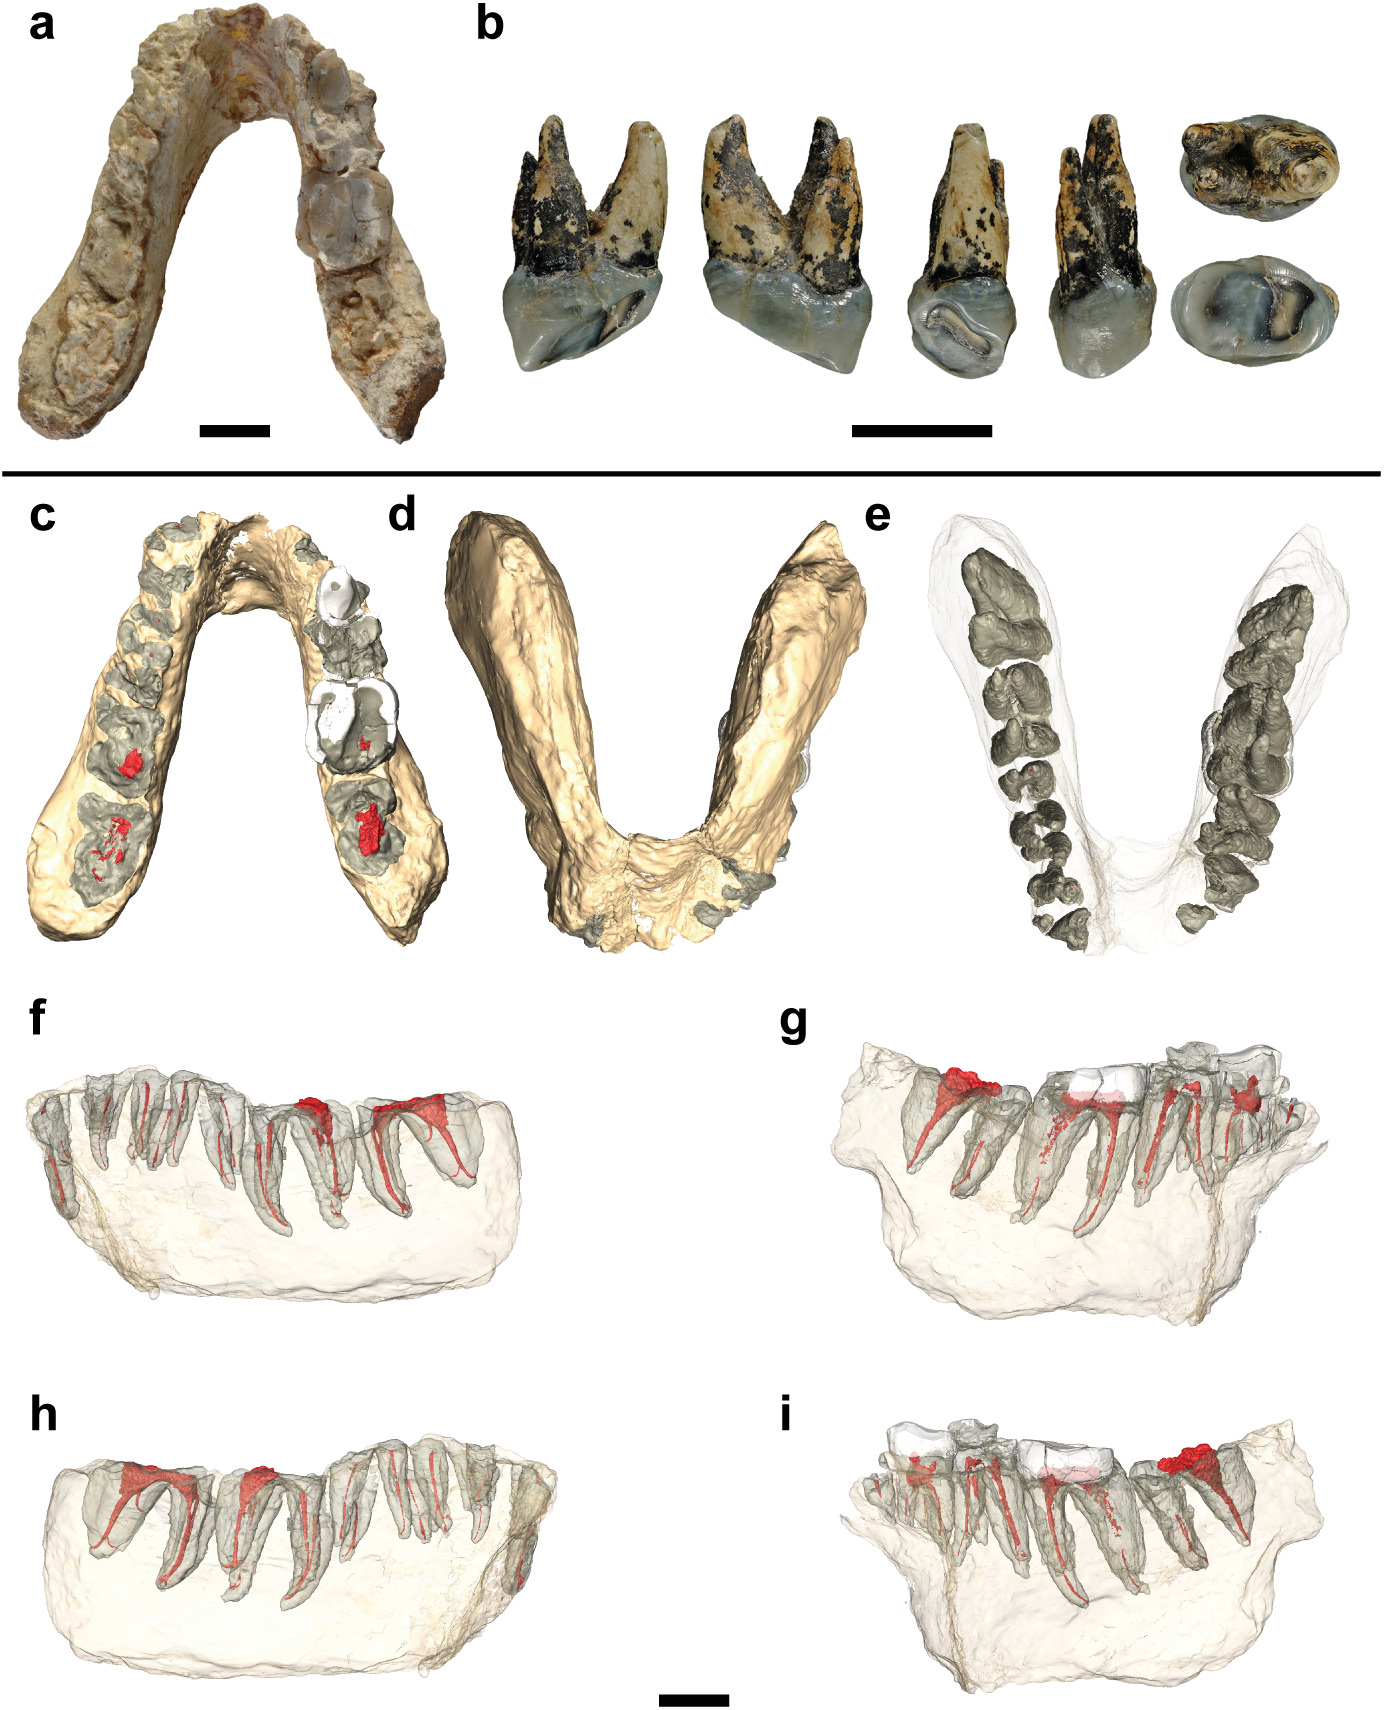
\includegraphics[width=0.3\textwidth]{Graecopithecus.jpg}
  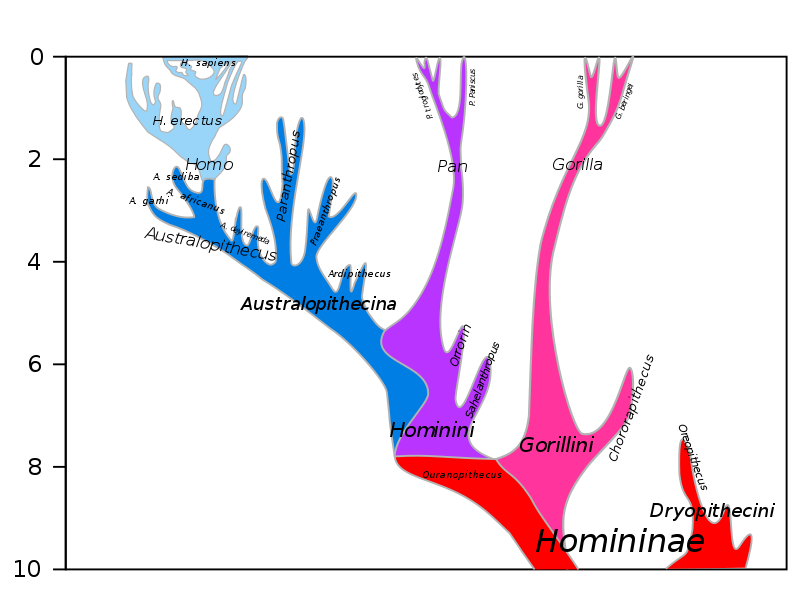
\includegraphics[width=0.5\textwidth]{Hominini_lineage.png}
  \caption{
    Left: El Graeco fossil, from \cite{fuss2017potential}.
    Right: Evolution of the Homininae, based on \cite{stringer2012makes}
 }
  \label{fig:human_evolution}
\end{figure}

Using fossils is a classic way to look back in evolutionary time.
Fossils show a glimpse of the biodiversity in the past.
We can deduce the age of fossils, by the rock layers they are found in.
Using fossils has its limitations. First, it is mostly species with hard body
parts that are suitable to fossilize. Of such species, an organisms is still 
only rarely preserved, of which only a fraction under ideal circumstances. Of 
these fossils, only a fraction is discovered.
One example of a famous fossil is 'El Graeco', 
which may be the oldest known hominin \cite{fuss2017potential}, where
homonins are the tribe (taxanomic group) we Homo sapiens share with the Panini.

% [picture of adaptive radiation phylogeny] | [picture of DDD phylogeny]
%                                           |
% An adaptive radiation.                    | The number of species through time.
%                                           | [use Etienne, DDD]



Using molecular phylogenies is the modern way to look back in evolutionary time.
It is the use of heritable molecules (e.g. DNA, RNA, or protein)  
of contemporary species to infer phylogenies. 
The field of phylogenetics is the research discipline that
intends to infer the most accurate phylogenies possible, 
regarding topology, speciation and extinction times,
optionally adding morphological data and/or fossil data.
Phylogenetics is applied in many settings, among
others, species classification,
forensics, conservation ecology
and epidemiology \cite{lam2010use}.

One example of the importance of an accurate phylogenetic tree 
is demonstrated in \cite{bush1999positive}. This study
investigated which loci of the H3 hemagglutinin surface protein
are under selection, by constrasting asynonymous and synonymous
mutation rates along the branches of a phylogeny. 
In a preliminary analysis by the authors, they noted that
most selection rates were either below or above the 
statistical threshold depending on the phylogeny.
This study contributed to the selection of recommended 
composition of influenza virus vaccines.

\begin{figure}[H]
  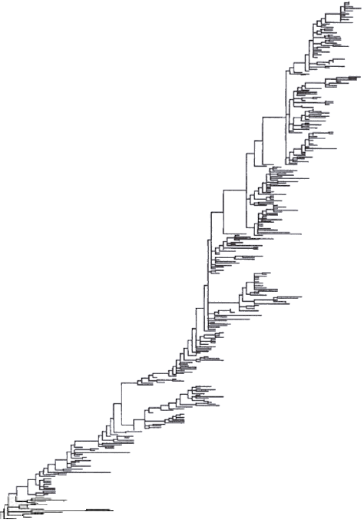
\includegraphics[width=0.3\textwidth]{bush_et_al_1999}
  %
  % A nice tree 
  %
  \caption{
    Phylogeny of the human influenza virus type A subtype H3,
    from \cite{bush1999positive}
  }
  \label{fig:bush_et_al_1999}
\end{figure}

\begin{figure}[H]
  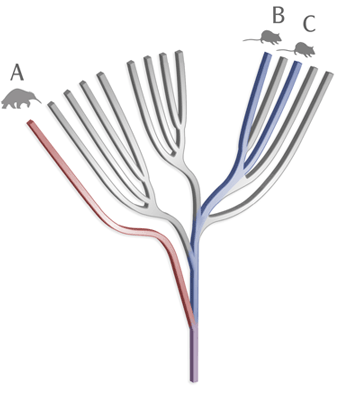
\includegraphics[width=0.3\textwidth]{edge_tree.png}
  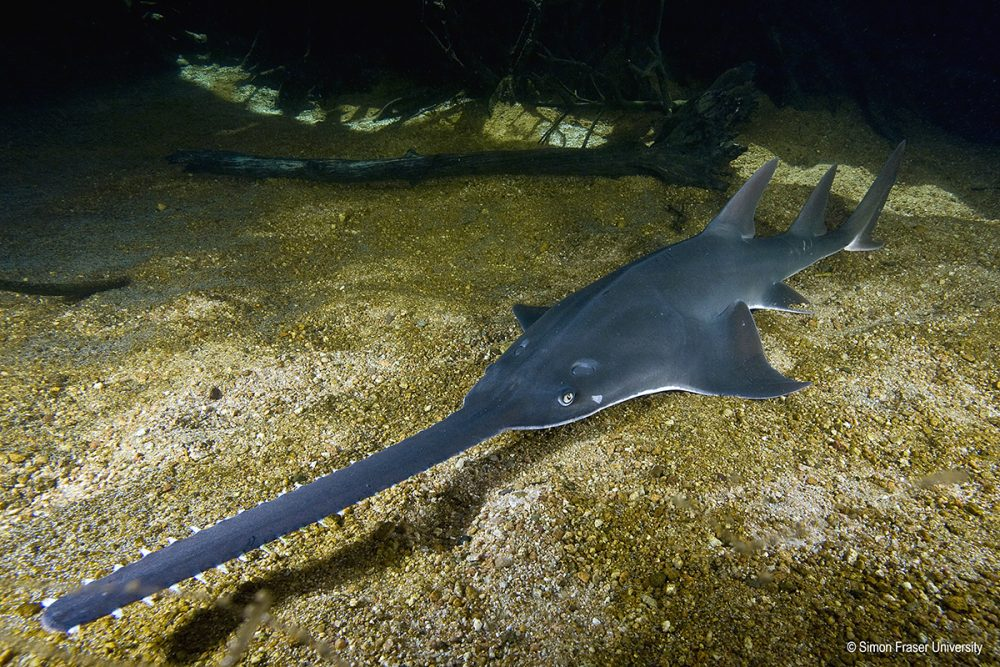
\includegraphics[width=0.5\textwidth]{Pristis-pristis_Simon-Fraser-University-1000x667.jpg}
  \caption{
    Left: The ED (evolutionary distinctiveness)       
    of species A is higher than that of species 
    B or C, as more                             
    evolutionary history will be lost when      
    that species goes extinct.
    Right: The Largetooth Sawfish (Pristis pristis) is at number 1 of the 
    EDGE (ED = 'Evolutionary Distinctiveness', GE = Globally Endangered status) 
    list, with an EDGE Score of 7.38 and an ED of 99.298.
 }
  \label{fig:edge_species}
\end{figure}

Another example of the importance of an accurate phylogenetic tree 
comes from conservation biology, in which phylogenies are used to
calculate an EDGE ('Evolutionarily Distinct and Globally Endangered') 
score. Species with a high EDGE score are prioritized in conservation.
To calculate an EDGE score, one needs a metric of evolutionary 
distinctiveness ('ED') and globally 'endangeredness' ('GE').
The GE score is a conservational status, ranging from from zero ('Least Concern') 
to four ('Critically Endangered'). 
The ED embodies the amount of evolutionary history lost when a species 
would go extinct, which can be calculated from a (hopefully accurate) 
phylogeny.

\begin{figure}[H]
  
\includegraphics[width=0.1\textwidth]{phylip.png}
  \caption{
    PHYLIP logo
 }
  \label{fig:phylip}
\end{figure}

Phylogenetics has taken a huge flight, due to the massively increased
computational power and techniques. A first milestone in this file is 
Felsensteyn's work in 1980, creating (and still maintaining) PHYLIP, 
the first software package for classical phylogenetic analysis.
Another milestone is the Metropolis-Hasting algorithm, which 
allowed Bayesian phylogenetics to thrive, resulting in
contemporay tools such as BEAST, BEAST2, MrBayes and RevBayes.

\begin{figure}[H]
  
\includegraphics[width=0.2\textwidth]{beast_logo.png}
  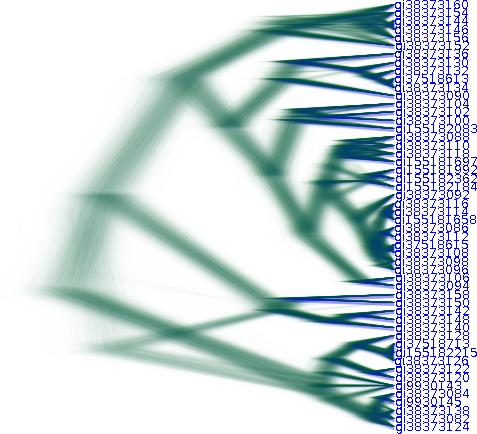
\includegraphics[width=0.2\textwidth]{DensiTreeExample2.jpg}
  \caption{
    BEAST2 logo (left) and example output (right)
 }
  \label{fig:beast2}
\end{figure}

A clear example of the power of modern phylogenetics,
is the Tree Of Life: it uses 
3,083 genomes of 2,596 amino-acid positions 
to create one big phylogeny of all (sequenced) life on Earth,
which took 3,840 computational hours on a modern supercomputer \cite{hug2016new}.


\begin{figure}[H]
  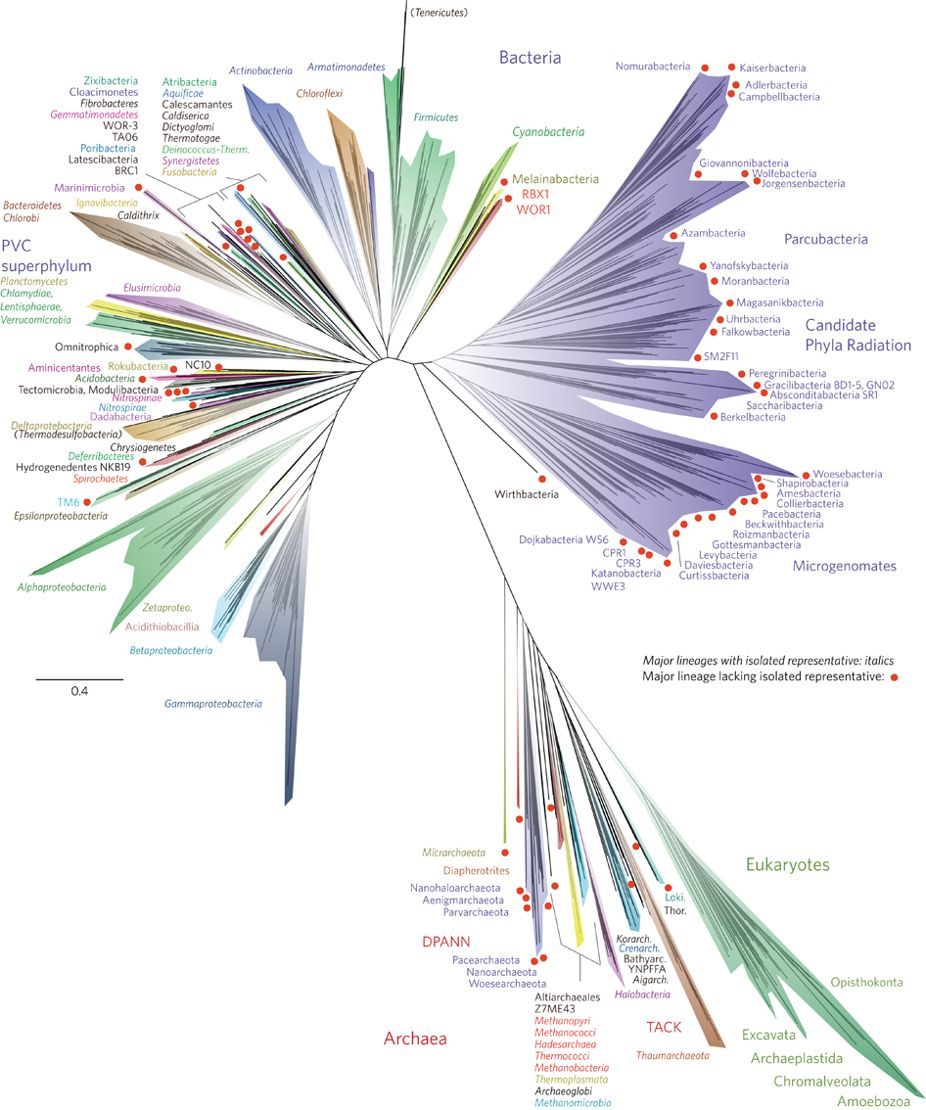
\includegraphics[width=0.4\textwidth]{tree_of_life_2016.jpg}
  \caption{
    Tree of Life, from \cite{hug2016new}
 }
  \label{fig:tree_of_life}
\end{figure}

To create such a tree from protein sequences, one has to specify
an evolutionary model. This evolutionary model embodies our set of
assumptions,
such as the evolution of a protein sequence (also called the site model), 
the rate(s) at which this happens (the clock model) 
and the rate(s) at which a branching/speciation event takes 
place (the tree model). 
For example, the amino acids of the Tree Of Life are assumed to change/mutate
according to the LG model \cite{le2008improved}, 
which is a model that uses the average transition rates found in nature.

There are many evolutionary models to choose from, 
and selecting which one to use is hard, due to the many sets of assumptions
to choose from. In general, modellers are looking for that set of assumptions
that is as simple as possible, but not simpler. And even then, sometimes
an overly simplistic model is picked regardless, due to computation 
constraints. 

By using a model comparison, one has a rational way to select 
an evolutionary model that is as simple as possible, but not simpler.
A model comparison algorithm selects the evolutionary model that is
most likely to have generated the data, without being overly complex.
The idea is that the best evolutionary model should result in the
most accurate phylogenetic trees.

Because model comparison is hard, there have been multiple
studies that investigate the effect of picking the wrong
evolutionary models. 

\begin{figure}[H]
  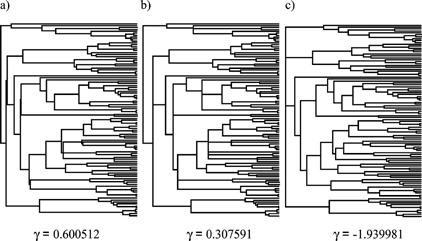
\includegraphics[width=0.5\textwidth]{revell2005under.png}
  \caption{
    Figure from \cite{revell2005under}. At the left was the true tree.
    In the middle the inferred tree, that used the generative model
    At the left the inferred tree when using a too simple inference model 
 }
  \label{fig:revell2005under}
\end{figure}

One example that demonstrates the effect of using a too simple inference model
comes from Revell at al \cite{revell2005under}.
They simulated many phylogenies and respective DNA sequences 
using different DNA substitution models. 
After this, they inferred phylogenies from the simulated alignments
with either the correct or a simpler DNA substitution model. 
Ideally, the inferred phylogenies match the phylogenies the alignments are based upon.
They found that when the DNA model is the correct one, inference of the
phylogenies is satisfactory.
However, when using an overly simplistic DNA model, 
the inferred trees show a slowdown in their speciation rates, 
also when the original trees were simulated with a constant speciation rate.
This study shows that a decreasing speciation rate may be attributed
to an overly simplistic DNA model, instead of an interesting biological process.

%
% [part of LG transition rate matrix]
% lg_transition_matrix.txt
%
% Part of an LG transition rate matrix

A more recent example that demonstrates the effect of using a too simple 
inference model is about assuming a wrong clock model. 
A clock model embodies our assumptions regarding the mutation rates in
the history of different taxa. The simplest clock model, called the strict
clock model, assumes these mutation rates are equal across all taxa.
Using a wrong clock model has a profound impact 
on the inferred phylogenetic trees, unless we can
specify the timing of some early speciation events \cite{duchene2014impact}.

\begin{figure}[H]
  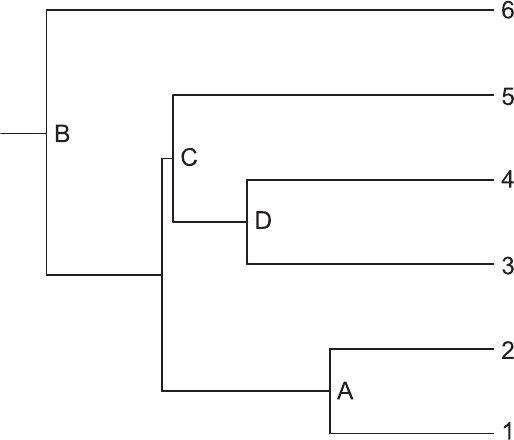
\includegraphics[width=0.3\textwidth]{duchene_et_al_2014_fig_1.png}
  \caption{
    Phylogeny with speciation events labelled A to D,
    where B is the earliest speciation event.
    Figure from \cite{duchene2014impact}.
 }
  \label{fig:duchene2014impact}
\end{figure}

The tree model is the most important piece of an evolutionary model,
with regard to speciation. The assumptions of a tree model is 
called the tree prior, where 'prior' refers to the knowledge
known before creating a phylogeny. The tree prior specifies how likely
processes that determine the shape of a tree occur. These
two processes are the formation of a new branch and the termination of
an existing branches. In the context of speciation, we call these
two events a speciation and an extinction event respectively.

There are two standard tree models, called the Yule (also: pure-birth(
and (standard) birth-death model. The most basic speciation model
is the Yule model [Yule, 19..] which assumes that speciation
is constant and there is no extinction.
[Research on fossils with Yule model would be fun].
The Yule model predict that the number of extant species
grows exponentially through time.

%
% [example Yule tree]  | [LTT plot for Yule model]
%                      |
% An example Yule tree | A lineages-through-time plot of the Yule model.
%                      | 

The Birth-Death model [Nee et al., 1994] is an extension of the
Yule that allows for a constant extinction rate. 
If the speciation rate exceeds the extinction rate,
also the BD model predicts that the number of extant species
grows exponentially through time. If the extinction rate exceeds
the speciation rate, the number of lineages is expected to decline
exponentially. The latter is biologically irrelevant.

%
% [example BD tree]  | [LTT plot for BD model]
%                    |
% An example BD tree | A lineages-through-time plot of the BD model.
%                    | 

It is clear that an exponential growth in the expected number of lineages
is biologically nonsense. 
To state the obvious: a finite area (Earth) results in a finite number of species. 
Applying the BD model to molecular data already shows that it does not
always hold, see figure [below]

%
% n_lineages
%
%   |      _______________
%   |   __/
%   | _/
%   |/
%   +---------------------
%
%       time
%
% An LTT plot for bird/lizards from [Etienne and Haegeman, 2012]
%

\begin{figure}[H]
  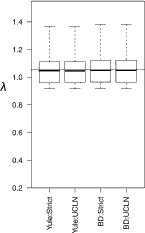
\includegraphics[width=0.2\textwidth]{sarver2019choice_top_4_bars.png}
  \caption{
    Estimation of the speciation rate (lambda)
    on inferred trees using 4 evolutionary models.
    The original trees had 100 taxa and were simulated with a strict clock model 
    and BD tree model, with a speciation rate of 1.104.
    Adapted from \cite{sarver2019choice}.
 }
  \label{fig:sarver2019choice}
\end{figure}

A recent study that investigates the effect of picking
a wrong standard tree prior, comes from Sarver et al, 2019 \cite{sarver2019choice}.
In this study, they first simulate trees using either a Yule or a birth-death
tree model, after which they simulate an alignment from that phylogeny
using two different standard clock models. From these alignments, 
they inferred the original trees using all of the four 
different clock and tree prior combinations. 
They show that, regardless which priors are used,
the estimated speciation and diversification rates 
from the inferred trees are similar to those of the original tree.

This thesis investigates the effect of picking a wrong standard
tree prior, when the tree is generated by a non-standard, novel tree model.
I will described the two new biological tree models that have been
investigated, as well as the re-usable framework to do so. 

The first novel and non-standard tree model is the protracted birth-death
model (PBD) \cite{etienne2012prolonging}.
Where the standard BD models assume that a speciation event creates
two new species instantly, the PBD model assumes that one of these two species
is an incipient species. An incipient species is a new species
that is not yet recognized as such, although complete reproductive
isolation is already present.
A biological example is from \cite{fennessy2013mitochondrial} in which
some new giraffe species have been discovered by sequencing
part of their DNA. Although these new species have been
'discovered' recently, the had been no gene flow between species
for already two million years.

Using the BD model in species that are slow to speciate, will cause
an underestimation of the number of lineages in the present (as in the
giraffes), in effect possibly giving the illusion that speciation 
slows down, where in reality it does not. 

\begin{figure}[H]

  %
  % n_lineages
  %
  %   |      _______________
  %   |   __/
  %   | _/
  %   |/
  %   +---------------------
  %
  %       time
  %
  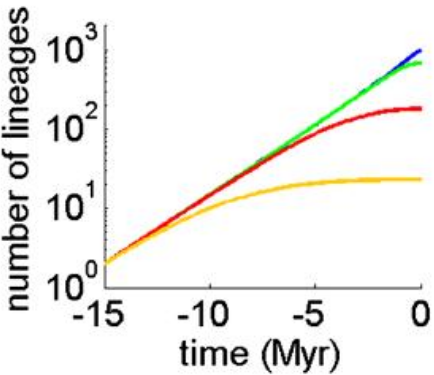
\includegraphics[width=0.3\textwidth]{eteinne_rosindell_2011_ltt.png}
  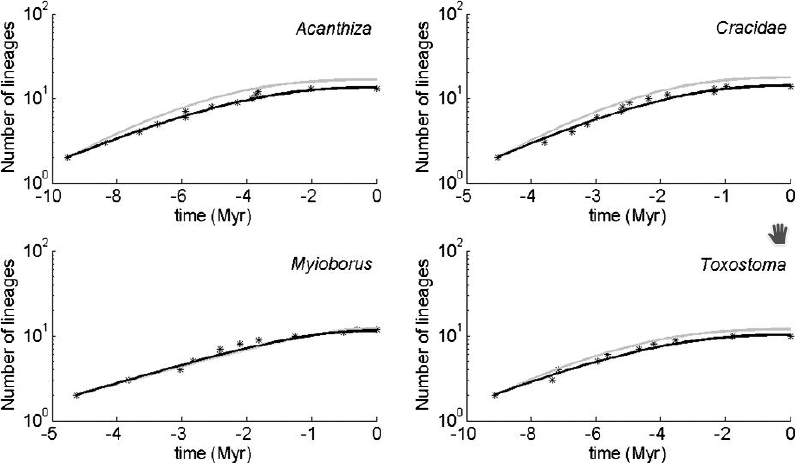
\includegraphics[width=0.5\textwidth]{eteinne_rosindell_2011.png}
  \caption{
    Left: example lineage-through-time plots, for different 
    speciation completion rates: yellow = 0.01, red = 0.1, green = 1.0, blue = 10.
    Note the slowdown in the accumulation of new lineages when speciation completion
    rate is lowered.
    Right: number of species through time plots for four bird phylogenies, 
    (after \cite{phillimore2008density})
    Both figures are adapted from \cite{etienne2012prolonging}
 }
  \label{fig:etienne2012prolonging}
\end{figure}

The second novel and non-standard tree model is the multiple-birth 
death (MBD) model [Laudanno et al., 2020].
Where the standard BD models assume that a speciation event occurs in one
species only at a time, the MBD models allows for speciation events
to occur in multiple species at the same time.
The biological idea behind this model, is that when a 
habitat (lake or mountain range) gets split into two, 
this may trigger speciation events in multiple species
of both communities at the same time. 
This mechanism is posed as an
explanation for high biodiversity in lake Tangyanika,
where the water level rises and falls with ice ages,
splitting up and merging the lake again and again, 
triggering co-occurring speciation events each change. 

%
% [phylogeny from Lake Tangyanika, use reference from Giovanni's MBD article]
%
% Phylogeny from Lake Tangyanika
%

This thesis investigates the effect of picking a wrong standard
tree prior, when the tree is generated 
by the non-standard PBD (chapter 5) or MBD (chapter 4) tree model.
It does so, by using the same experimental setup, called 'pirouette',
which is described in chapter 3. This framework is built up a foundation
of R packages called 'babette', which is described in chapter 2.

\begin{figure}[H]
  \includegraphics[width=0.3\textwidth]{The_Earth_seen_from_Apollo_17.jpg}
  \caption{
    Environment that follows an unknown speciation model.
 }
  \label{fig:unknown_speciation_model}
\end{figure}

In the end, we want to know how well we can infer a phylogeny from
molecular data found in the field. That field, outside, 
which follows an unknown speciation model. Let us just hope our inference
is robust to whatever novel model we throw at it.

